% (find-LATEX "2023-1-C4-P1.tex")
% (defun c () (interactive) (find-LATEXsh "lualatex -record 2023-1-C4-P1.tex" :end))
% (defun C () (interactive) (find-LATEXsh "lualatex 2023-1-C4-P1.tex" "Success!!!"))
% (defun D () (interactive) (find-pdf-page      "~/LATEX/2023-1-C4-P1.pdf"))
% (defun d () (interactive) (find-pdftools-page "~/LATEX/2023-1-C4-P1.pdf"))
% (defun e () (interactive) (find-LATEX "2023-1-C4-P1.tex"))
% (defun o () (interactive) (find-LATEX "2023-1-C4-P1.tex"))
% (defun u () (interactive) (find-latex-upload-links "2023-1-C4-P1"))
% (defun v () (interactive) (find-2a '(e) '(d)))
% (defun d0 () (interactive) (find-ebuffer "2023-1-C4-P1.pdf"))
% (defun cv () (interactive) (C) (ee-kill-this-buffer) (v) (g))
%          (code-eec-LATEX "2023-1-C4-P1")
% (find-pdf-page   "~/LATEX/2023-1-C4-P1.pdf")
% (find-sh0 "cp -v  ~/LATEX/2023-1-C4-P1.pdf /tmp/")
% (find-sh0 "cp -v  ~/LATEX/2023-1-C4-P1.pdf /tmp/pen/")
%     (find-xournalpp "/tmp/2023-1-C4-P1.pdf")
%   file:///home/edrx/LATEX/2023-1-C4-P1.pdf
%               file:///tmp/2023-1-C4-P1.pdf
%           file:///tmp/pen/2023-1-C4-P1.pdf
%  http://anggtwu.net/LATEX/2023-1-C4-P1.pdf
% (find-LATEX "2019.mk")
% (find-Deps1-links "Caepro5 Piecewise1")
% (find-Deps1-cps   "Caepro5 Piecewise1")
% (find-Deps1-anggs "Caepro5 Piecewise1")
% (find-MM-aula-links "2023-1-C4-P1" "C4" "c4m231p1" "c4p1")

% «.defs»		(to "defs")
% «.defs-T-and-B»	(to "defs-T-and-B")
% «.defs-caepro»	(to "defs-caepro")
% «.defs-pict2e»	(to "defs-pict2e")
% «.title»		(to "title")
% «.links»		(to "links")
% «.questoes-123»	(to "questoes-123")
% «.dicas»		(to "dicas")
% «.questao-1-gab»	(to "questao-1-gab")
% «.questao-2-gab»	(to "questao-2-gab")
% «.questao-3-gab»	(to "questao-3-gab")
%
% «.djvuize»		(to "djvuize")



% <videos>
% Video (not yet):
% (find-ssr-links     "c4m231p1" "2023-1-C4-P1")
% (code-eevvideo      "c4m231p1" "2023-1-C4-P1")
% (code-eevlinksvideo "c4m231p1" "2023-1-C4-P1")
% (find-c4m231p1video "0:00")

\documentclass[oneside,12pt]{article}
\usepackage[colorlinks,citecolor=DarkRed,urlcolor=DarkRed]{hyperref} % (find-es "tex" "hyperref")
\usepackage{amsmath}
\usepackage{amsfonts}
\usepackage{amssymb}
\usepackage{pict2e}
\usepackage[x11names,svgnames]{xcolor} % (find-es "tex" "xcolor")
\usepackage{colorweb}                  % (find-es "tex" "colorweb")
%\usepackage{tikz}
%
% (find-dn6 "preamble6.lua" "preamble0")
%\usepackage{proof}   % For derivation trees ("%:" lines)
%\input diagxy        % For 2D diagrams ("%D" lines)
%\xyoption{curve}     % For the ".curve=" feature in 2D diagrams
%
\usepackage{edrx21}               % (find-LATEX "edrx21.sty")
\input edrxaccents.tex            % (find-LATEX "edrxaccents.tex")
\input edrx21chars.tex            % (find-LATEX "edrx21chars.tex")
\input edrxheadfoot.tex           % (find-LATEX "edrxheadfoot.tex")
\input edrxgac2.tex               % (find-LATEX "edrxgac2.tex")
%\usepackage{emaxima}              % (find-LATEX "emaxima.sty")
%
% (find-es "tex" "geometry")
\usepackage[a6paper, landscape,
            top=1.5cm, bottom=.25cm, left=1cm, right=1cm, includefoot
           ]{geometry}
%
\begin{document}

% «defs»  (to ".defs")
% (find-LATEX "edrx21defs.tex" "colors")
% (find-LATEX "edrx21.sty")

\def\drafturl{http://anggtwu.net/LATEX/2023-1-C4.pdf}
\def\drafturl{http://anggtwu.net/2023.1-C4.html}
\def\draftfooter{\tiny \href{\drafturl}{\jobname{}} \ColorBrown{\shorttoday{} \hours}}

\def\Dint{\int\!\!\!\!\int}
\def\P#1{\left( #1 \right)}

% «defs-T-and-B»  (to ".defs-T-and-B")
\long\def\ColorOrange#1{{\color{orange!90!black}#1}}
\def\T(Total: #1 pts){{\bf(Total: #1)}}
\def\T(Total: #1 pts){{\bf(Total: #1 pts)}}
\def\T(Total: #1 pts){\ColorRed{\bf(Total: #1 pts)}}
\def\B       (#1 pts){\ColorOrange{\bf(#1 pts)}}

% (find-LATEX "2023-1-C2-carro.tex" "defs-caepro")
% (find-LATEX "2023-1-C2-carro.tex" "defs-pict2e")

\catcode`\^^J=10
\directlua{dofile "dednat6load.lua"}  % (find-LATEX "dednat6load.lua")

% «defs-caepro»  (to ".defs-caepro")
%L dofile "Caepro5.lua"              -- (find-angg "LUA/Caepro5.lua" "LaTeX")
\def\Caurl   #1{\expr{Caurl("#1")}}
\def\Cahref#1#2{\href{\Caurl{#1}}{#2}}
\def\Ca      #1{\Cahref{#1}{#1}}

% «defs-pict2e»  (to ".defs-pict2e")
%L V = nil                           -- (find-angg "LUA/Pict2e1.lua" "MiniV")
%L dofile "Piecewise1.lua"           -- (find-LATEX "Piecewise1.lua")
%L Pict2e.__index.suffix = "%"
\def\pictgridstyle{\color{GrayPale}\linethickness{0.3pt}}
\def\pictaxesstyle{\linethickness{0.5pt}}
\def\pictnaxesstyle{\color{GrayPale}\linethickness{0.5pt}}
\celllower=2.5pt

\pu




%  _____ _ _   _                               
% |_   _(_) |_| | ___   _ __   __ _  __ _  ___ 
%   | | | | __| |/ _ \ | '_ \ / _` |/ _` |/ _ \
%   | | | | |_| |  __/ | |_) | (_| | (_| |  __/
%   |_| |_|\__|_|\___| | .__/ \__,_|\__, |\___|
%                      |_|          |___/      
%
% «title»  (to ".title")
% (c4m231p1p 1 "title")
% (c4m231p1a   "title")

\thispagestyle{empty}

\begin{center}

\vspace*{1.2cm}

{\bf \Large Cálculo C4 - 2023.1}

\bsk

Primeira prova (P1)

\bsk

Eduardo Ochs - RCN/PURO/UFF

\url{http://anggtwu.net/2023.1-C4.html}

\end{center}

\newpage

% «links»  (to ".links")


%   ___                  _                    _     ____      _____ 
%  / _ \ _   _  ___  ___| |_ ___   ___  ___  / |   |___ \    |___ / 
% | | | | | | |/ _ \/ __| __/ _ \ / _ \/ __| | |     __) |     |_ \ 
% | |_| | |_| |  __/\__ \ || (_) |  __/\__ \ | |_   / __/ _   ___) |
%  \__\_\\__,_|\___||___/\__\___/ \___||___/ |_( ) |_____( ) |____/ 
%                                              |/        |/         
% «questoes-123»  (to ".questoes-123")
% (c4m231p1p 2 "questoes-123")
% (c4m231p1a   "questoes-123")

\scalebox{0.65}{\def\colwidth{8.5cm}\firstcol{

{\bf Questão 1.}

\T(Total: 1.0 pts)

Seja $R$ o retângulo da direita.

Calcule:
%
$$\Dint_R x^3 y^5 \, dx \, dy.$$

Dica: neste caso tanto faz você integrar primeiro em $x$ e depois em
$y$ quanto integrar primeiro em $y$ e depois em $x$; os dois modos são
igualmente fáceis.


\bsk
\bsk

{\bf Questão 2.}

\T(Total: 5.0 pts)

Seja $B$ a região tipo ``pedaço de bolo'' à direita -- ela é um quarto de
um bolo de raio 2 com furo de raio 1. Calcule
%
$$\Dint_B x \, dx \, dy.$$

Pra resolver isso você vai ter que mudar a integral pra coordenadas
polares.

}\anothercol{

\vspace*{1cm}

% (find-latexscan-links "C4" "C4-P1-R")
% (find-latexscan-links "C4" "C4-P1-B")
% (find-xpdf-page "~/LATEX/2023-1-C4/C4-P1-R.pdf")
% (find-xpdf-page "~/LATEX/2023-1-C4/C4-P1-B.pdf")
$$\begin{array}{rcc}
  R &=& \myvcenter{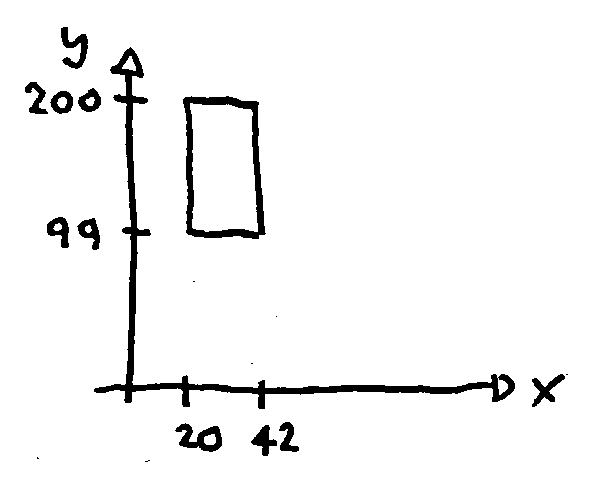
\includegraphics[height=3cm]{2023-1-C4/C4-P1-R.pdf}} \\
  B &=& \myvcenter{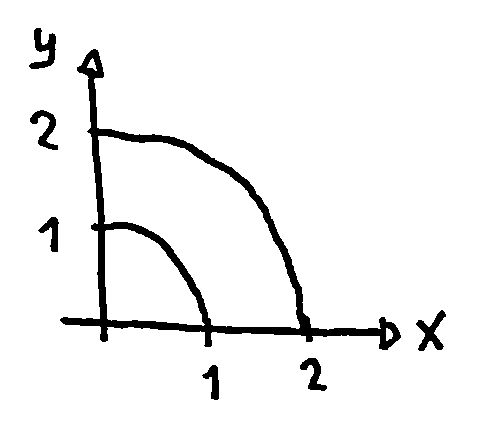
\includegraphics[height=2cm]{2023-1-C4/C4-P1-B.pdf}} \\
  \end{array}
$$

\vspace*{1cm}

{\bf Questão 3.}

\T(Total: 6.0 pts)

Seja $S$ este retângulo: $S = [1,2]×[1,2]$. Calcule esta integral de
linha:
%
$$\oint_{∂S} \VEC{xy^2,x^3y^4}·\VEC{dx,dy}.$$

}}


\newpage

%  ____  _               
% |  _ \(_) ___ __ _ ___ 
% | | | | |/ __/ _` / __|
% | |_| | | (_| (_| \__ \
% |____/|_|\___\__,_|___/
%                        
% «dicas»  (to ".dicas")


\scalebox{0.6}{\def\colwidth{9cm}\firstcol{

{}

{\bf Dica:} Pra ``calcular'' $\difx{23}{45}{x^3}$ basta fazer isso
aqui:
%
$$\difx{23}{45}{x^3} \;=\; 45^3 - 23^3$$

com isso você chega em algo que dá pra transformar num número usando
só uma calculadora que só saiba fazer operações básicas. Você não
precisa destes passos extras:
%
$$45^3 - 23^3 \;=\; 91125 - 12167 \;=\; 78958$$

A explicação está em um dos slides de Cálculo 2 do material anexo --
procure por ``dicas sobre simplificação''.


\bsk
\bsk

{\bf Outra dica.} Nas questões desta prova o que vai contar mais
pontos é você organizar as contas de modo que cada passo seja fácil de
entender, de verificar, e de justificar -- ``chegar no resultado
certo'' vai valer relativamente pouco.

}\anothercol{
}}


\newpage


\scalebox{0.7}{\def\colwidth{8cm}\firstcol{

% «questao-1-gab»  (to ".questao-1-gab")
% (c4m231p1p 4 "questao-1-gab")
% (c4m231p1a   "questao-1-gab")

{\bf Questão 1: gabarito}

\def\Intxx#1{\Intx{20}{42}{#1}}
\def\Intyy#1{\Inty{99}{200}{#1}}
\def\difxx#1{\difx{20}{42}{#1}}
\def\difyy#1{\difx{99}{200}{#1}}

$$\begin{array}{l}
  \int \!\!\! \int_R x^3 y^5 \, dx \, dy \\
  =\;\; \Intxx{\Intyy{x^3 y^5}} \\
  =\;\; \Intxx{x^3 \P{\Intyy{y^5}}} \\
  =\;\; \P{\Intxx{x^3}}
        \P{\Intyy{y^5}} \\
  =\;\; \P{\difxx{\frac{x^4}{4}}}
        \P{\difyy{\frac{y^6}{6}}} \\\\[-8pt]
  =\;\; \frac{42^4-20^4}{4} \;
        \frac{200^6-99^6}{6}
  \end{array}
$$



}\anothercol{

% «questao-2-gab»  (to ".questao-2-gab")
% (c4m231p1p 4 "questao-2-gab")
% (c4m231p1a   "questao-2-gab")

{\bf Questão 2: gabarito}

\def\vmat#1{\left| \begin{matrix}     #1\end{matrix}      \right|}
\def\vsm #1{\left| \begin{smallmatrix}#1\end{smallmatrix} \right|}
\def\Intrr#1{\Intr {1}{2}{#1}}
\def\Inttt#1{\Intth{0}{\frac{π}{2}}{#1}}
\def\difrr#1{\difr {1}{2}{#1}}
\def\diftt#1{\difth{0}{\frac{π}{2}}{#1}}

Vamos usar esta mudança de variáveis:
%
$$\begin{array}{rcl}
  (x,y) &=& (r\cosθ, r\senθ) \\
  \vsm{x_r & x_θ \\ y_r & y_θ}
    &=& \vsm{\cosθ & r(-\senθ) \\ \senθ & r\cosθ}
        \;=\; r  \\
  % &=& r  \\
  dx\,dy &=& \vsm{x_r & x_θ \\ y_r & y_θ} dr\,dθ \\
         &=& r\,dr\,dθ \\
  \end{array}
$$

Então:

$$\begin{array}{l}
  \int \!\!\! \int_B x \, dx \, dy \\
  =\;\; \Intrr{\Inttt{(r\cosθ)\,r}} \\
  =\;\; \Intrr{\Inttt{r^2\cosθ}}                    \\
  =\;\; \P{\Intrr{r^2}} \P{\Inttt{\cosθ}}           \\
  =\;\; \P{\difrr{\frac{r^3}{3}}} \P{\diftt{\senθ}} \\
  =\;\; \frac{8-1}{3}(1-0) \\
  \end{array}
$$


}}


\newpage

% «questao-3-gab»  (to ".questao-3-gab")
% (c4m231p1p 5 "questao-3-gab")
% (c4m231p1a   "questao-3-gab")

\def\Inttp#1{\Intt{ 1}{ 2}{#1}}
\def\Inttn#1{\Intt{-2}{-1}{#1}}
\def\diftp#1{\dift{ 1}{ 2}{#1}}
\def\diftn#1{\dift{-2}{-1}{#1}}

\scalebox{0.45}{\def\colwidth{6cm}\firstcol{

{\bf Questão 3: gabarito}

Vou decompor $∂S$ em $C_1$, $C_2$, $C_3$, $C_4$ -- as paredes direita,
de cima, esquerda, e de baixo do quadrado -- e vou parametrizar $C_1$,
$C_2$, $C_3$, $C_4$ desta forma:

\msk

Em $C_1$: $(x(t),y(t))=(2,t)$,

com $t$ indo de $1$ até 2;

aqui $(x_t,y_t)=(0,1)$.

\msk

Em $C_2$: $(x(t),y(t))=(-t,2)$,

com $t$ indo de $-2$ até -1;

aqui $(x_t,y_t)=(-1,0)$.

\msk

Em $C_3$: $(x(t),y(t))=(1,-t)$,

com $t$ indo de $-2$ até -1;

aqui $(x_t,y_t)=(0,-1)$.

\msk

Em $C_4$: $(x(t),y(t))=(t,1)$,

com $t$ indo de $1$ até 2;

aqui $(x_t,y_t)=(1,0)$.

\ssk



}\anothercol{

\vspace*{0.2cm}

Temos:

\msk

$\begin{array}{l}
  \int_{C_1} (P,Q)·(dx,dy) \\
  =\; \Inttp {(P,Q)·(x_t,y_t)} \\
  =\; \Inttp {(P,Q)·(0,1)} \\
  =\; \Inttp {Q(x(t),y(t))} \\
  =\; \Inttp {Q(2,t)} \\
  \\
  \int_{C_2} (P,Q)·(dx,dy) \\
  =\; \Inttn {(P,Q)·(x_t,y_t)} \\
  =\; \Inttn {(P,Q)·(-1,0)} \\
  =\; \Inttn {-P(x(t),y(t))} \\
  =\; \Inttn {-P(-t,2)} \\
  \\
  \int_{C_3} (P,Q)·(dx,dy) \\
  =\; \Inttn {(P,Q)·(x_t,y_t)} \\
  =\; \Inttn {(P,Q)·(0,-1)} \\
  =\; \Inttn {-Q(x(t),y(t))} \\
  =\; \Inttn {-Q(1,-t)} \\
  \\
  \int_{C_4} (P,Q)·(dx,dy) \\
  =\; \Inttp {(P,Q)·(x_t,y_t)} \\
  =\; \Inttp {(P,Q)·(1,0)} \\
  =\; \Inttp {P(x(t),y(t))} \\
  =\; \Inttp {P(t,1)} \\
  \end{array}
$

% $$\Inttp{\Inttn{foo}}$$

}\anothercol{

\vspace*{0.2cm}

Como nesse problema temos

$P(x,y) = xy^2$ e $Q(x,y) = x^3y^4$,

isso vira:

\msk

$\begin{array}{l}
  \int_{C_1} (P,Q)·(dx,dy) \\
  =\; \Inttp {Q(2,t)} \\
  =\; \Inttp {2^3t^4} \\
  =\; 2^3 \Inttp {t^4} \\
  =\; 8 \P{\diftp {\frac{t^5}{5}}} \\
  \\
  \int_{C_2} (P,Q)·(dx,dy) \\
  =\; \Inttn {-P(-t,2)} \\
  =\; \Inttn {-(-t)2^2} \\
  =\; 4 \Inttn {t} \\
  =\; 4 \P{\diftn {\frac{t^2}{2}}} \\
  \\
  \int_{C_3} (P,Q)·(dx,dy) \\
  =\; \Inttn {-Q(1,-t)} \\
  =\; \Inttn {-1^3(-t)^4} \\
  =\; - \Inttn {t^4} \\
  =\; 4 \P{\diftn {\frac{t^5}{5}}} \\
  \\
  \int_{C_4} (P,Q)·(dx,dy) \\
  =\; \Inttp {P(t,1)} \\
  =\; \Inttp {t·1^2} \\
  =\; \Inttp {t} \\
  =\; \P{\diftp {\frac{t^2}{2}}} \\
  \end{array}
$

}\anothercol{

\vspace*{0.2cm}

E aí:

\msk

$\begin{array}{l}
  \oint_{∂S} (xy^2,x^3y^4)·(dx,dy) \\
  = \; \int_{C_1} (xy^2,x^3y^4)·(dx,dy) \\
  + \; \int_{C_2} (xy^2,x^3y^4)·(dx,dy) \\
  + \; \int_{C_3} (xy^2,x^3y^4)·(dx,dy) \\
  + \; \int_{C_4} (xy^2,x^3y^4)·(dx,dy) \\
  = \; 8 \P{\diftp {\frac{t^5}{5}}} \\
  + \; 4 \P{\diftn {\frac{t^2}{2}}} \\
  + \; 4 \P{\diftn {\frac{t^5}{5}}} \\
  + \;   \P{\diftp {\frac{t^2}{2}}} . \\
  \end{array}
$

}}




% (find-es "maxima" "2023-1-C4-P1")


\GenericWarning{Success:}{Success!!!}  % Used by `M-x cv'

\end{document}

%  ____  _             _         
% |  _ \(_)_   ___   _(_)_______ 
% | | | | \ \ / / | | | |_  / _ \
% | |_| | |\ V /| |_| | |/ /  __/
% |____// | \_/  \__,_|_/___\___|
%     |__/                       
%
% «djvuize»  (to ".djvuize")
% (find-LATEXgrep "grep --color -nH --null -e djvuize 2020-1*.tex")

 (eepitch-shell)
 (eepitch-kill)
 (eepitch-shell)
# (find-fline "~/2023.1-C4/")
# (find-fline "~/LATEX/2023-1-C4/")
# (find-fline "~/bin/djvuize")

cd /tmp/
for i in *.jpg; do echo f $(basename $i .jpg); done

f () { rm -v $1.pdf;  textcleaner -f 50 -o  5 $1.jpg $1.png; djvuize $1.pdf; xpdf $1.pdf }
f () { rm -v $1.pdf;  textcleaner -f 50 -o 10 $1.jpg $1.png; djvuize $1.pdf; xpdf $1.pdf }
f () { rm -v $1.pdf;  textcleaner -f 50 -o 20 $1.jpg $1.png; djvuize $1.pdf; xpdf $1.pdf }

f () { rm -fv $1.png $1.pdf; djvuize $1.pdf }
f () { rm -fv $1.png $1.pdf; djvuize WHITEBOARDOPTS="-m 1.0 -f 15" $1.pdf; xpdf $1.pdf }
f () { rm -fv $1.png $1.pdf; djvuize WHITEBOARDOPTS="-m 1.0 -f 30" $1.pdf; xpdf $1.pdf }
f () { rm -fv $1.png $1.pdf; djvuize WHITEBOARDOPTS="-m 1.0 -f 45" $1.pdf; xpdf $1.pdf }
f () { rm -fv $1.png $1.pdf; djvuize WHITEBOARDOPTS="-m 0.5" $1.pdf; xpdf $1.pdf }
f () { rm -fv $1.png $1.pdf; djvuize WHITEBOARDOPTS="-m 0.25" $1.pdf; xpdf $1.pdf }
f () { cp -fv $1.png $1.pdf       ~/2023.1-C4/
       cp -fv        $1.pdf ~/LATEX/2023-1-C4/
       cat <<%%%
% (find-latexscan-links "C4" "$1")
%%%
}

f C4-P1-B
f C4-P1-R

f 20230612_012330

f 20201213_area_em_funcao_de_theta
f 20201213_area_em_funcao_de_x
f 20201213_area_fatias_pizza


% Local Variables:
% coding: utf-8-unix
% ee-tla: "c4p1"
% ee-tla: "c4m231p1"
% End:
